% $Id: introduction.tex 87303 2016-02-08 13:44:29Z lafferty $

\subsection{Background sources}
\label{subsec:background}

Several sources of background are investigated to assess their relevance for a measurement of \BRof\Kspizmm:
\begin{itemize}
%\item Misidentified \Kspipi decays (combined with a combinatorial $\pi^0$ in the case of FULL). 
\item \Kspipi decays, where both pions are misidentified as muons, and in the case of the FULL category, combined with a random $\pi^0$ from the underlying event.
These decays have a mass larger than that of the \KS and do not enter the fit region, except for potential residual tails that effectively add up to the combinatorial background. % TODO (see \figref{fig:Kspipibkg}). 
No evidence for \Kspipi background is seen for the BDT region being fitted. 
\item \KTmTg decays. This background was considered in the NA48 analysis ~\cite{NA48}, 
However, its contribution at LHCb is found to be negligible: In the case of the \KL decay (with a branching fraction of $1.0^{+0.8}_{-0.6}\times10^{-8}$ ~\cite{PDG}) the upper decay time acceptance introduces 
an effective $10^{-3}$ reduction with respect to \KS and hence
the effective \BRof\KLTmTg becomes as low as $10^{-11}$. There is no experimental measurement of \BRof\KSTmTg, however, since
the process is dominated by the two-photon exchange\footnote{Isidori and D'Ambrosio, private communication.}, it can be estimated as:
\begin{equation}
\BRof\KSTmTg = \frac{\BRof\KSTg}{\BRof\KLTg}\BRof\KLTmTg \sim 4.8\times10^{-11}
\end{equation} 
\noindent and is thus negligible.
\item \KLTpi decays. The mass distribution of these decays is shown in \figref{fig:KLTpi} as obtained in simulation. Since there is no evidence of this background in the 
data, it is neglected. Including a \KLTpi component to the observed background does not change significantly the sensitivity estimates. The \KS counterpart has a branching fraction of $3.5\times10^{-7}$ and thus
is about four orders of magnitude smaller than \KLTpi. In general, no sign of a resonant structure in the $\pi^+\pi^-\pi^0$ is seen on data.

\item Combinatorial background. Combinatorial background is considered to be composed by random combination of tracks, including those generated by pseudo-random combinations of hits during the pattern recognition. 
It has a monotonic shape across the studied invariant mass range.

\end{itemize}

\begin{figure} [htb!]
\begin{center}
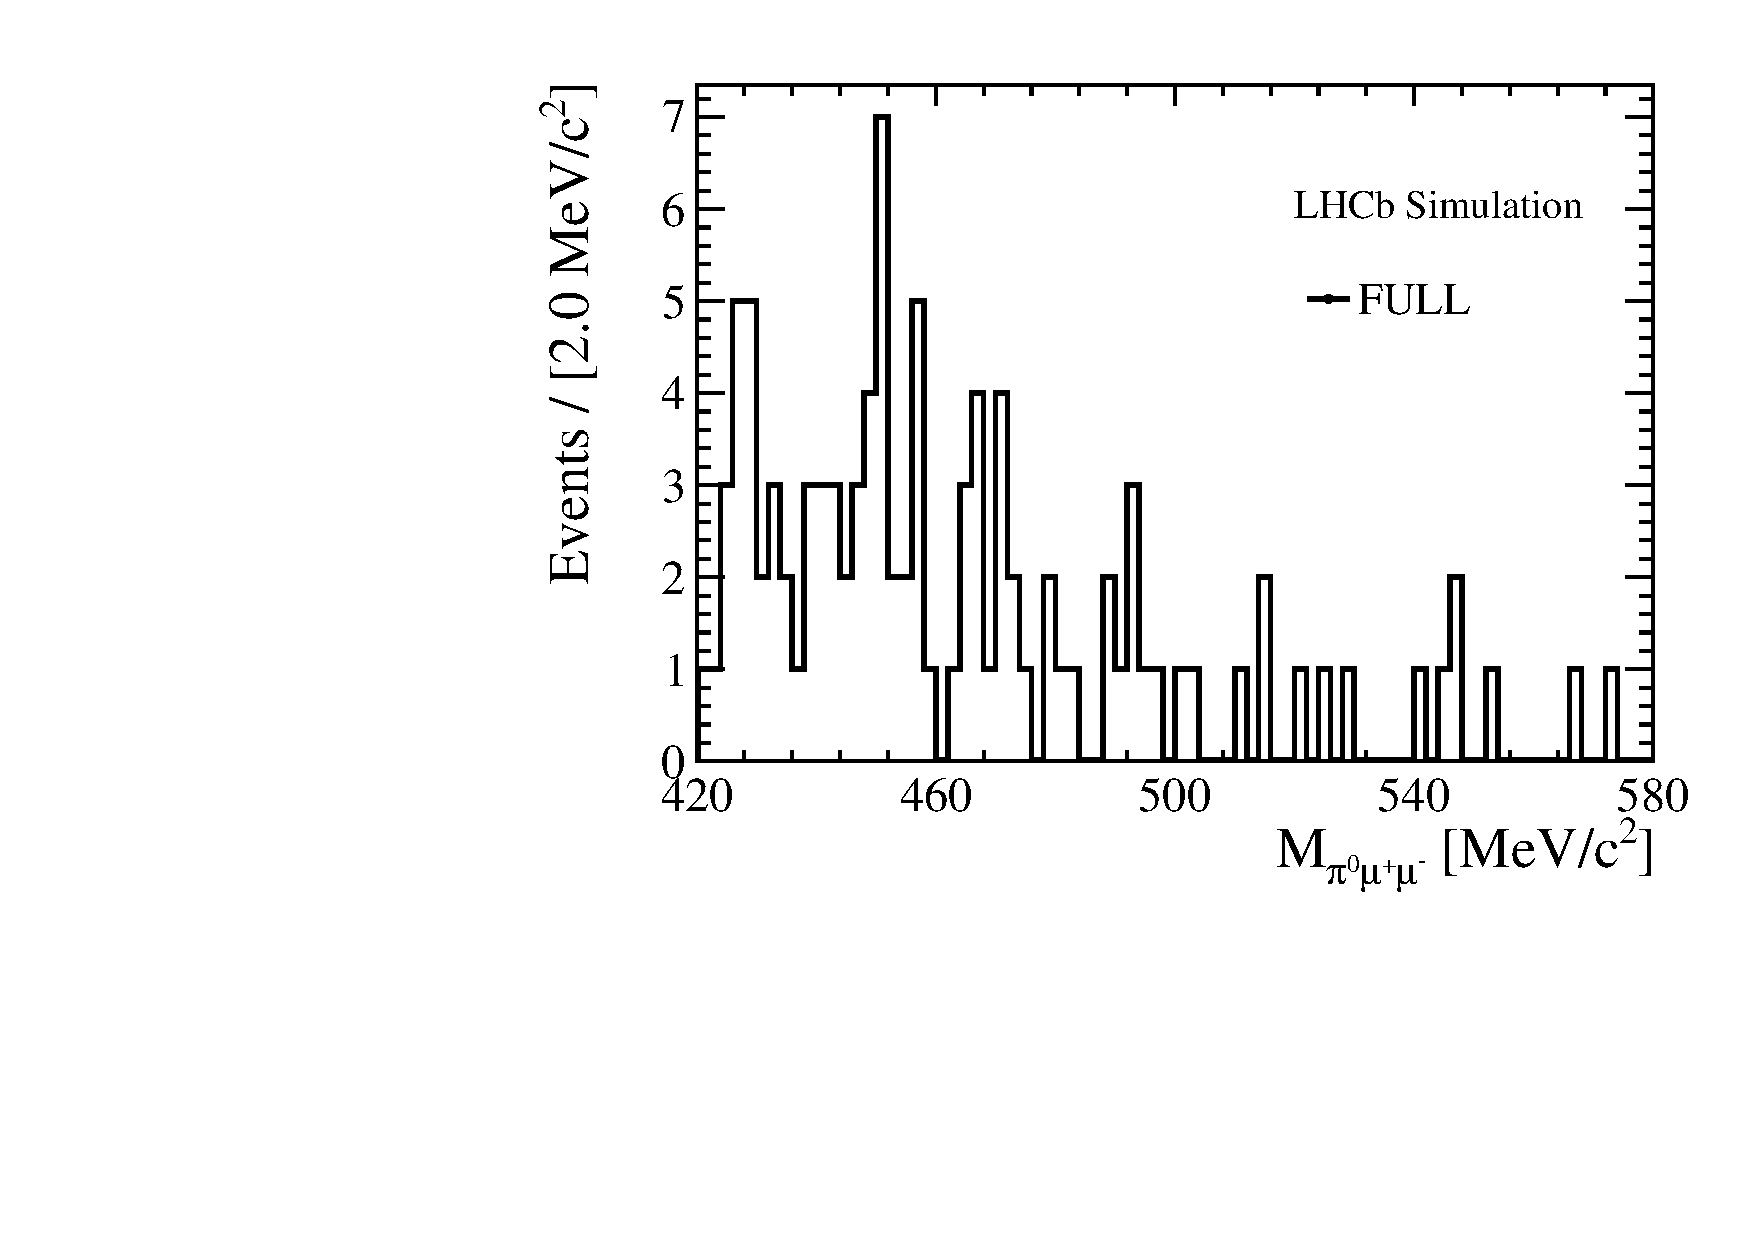
\includegraphics[scale=0.30]{figs/Kspi0MuMu/M_VC_K3pi.pdf}%{figs/K3pi_FULL.pdf}
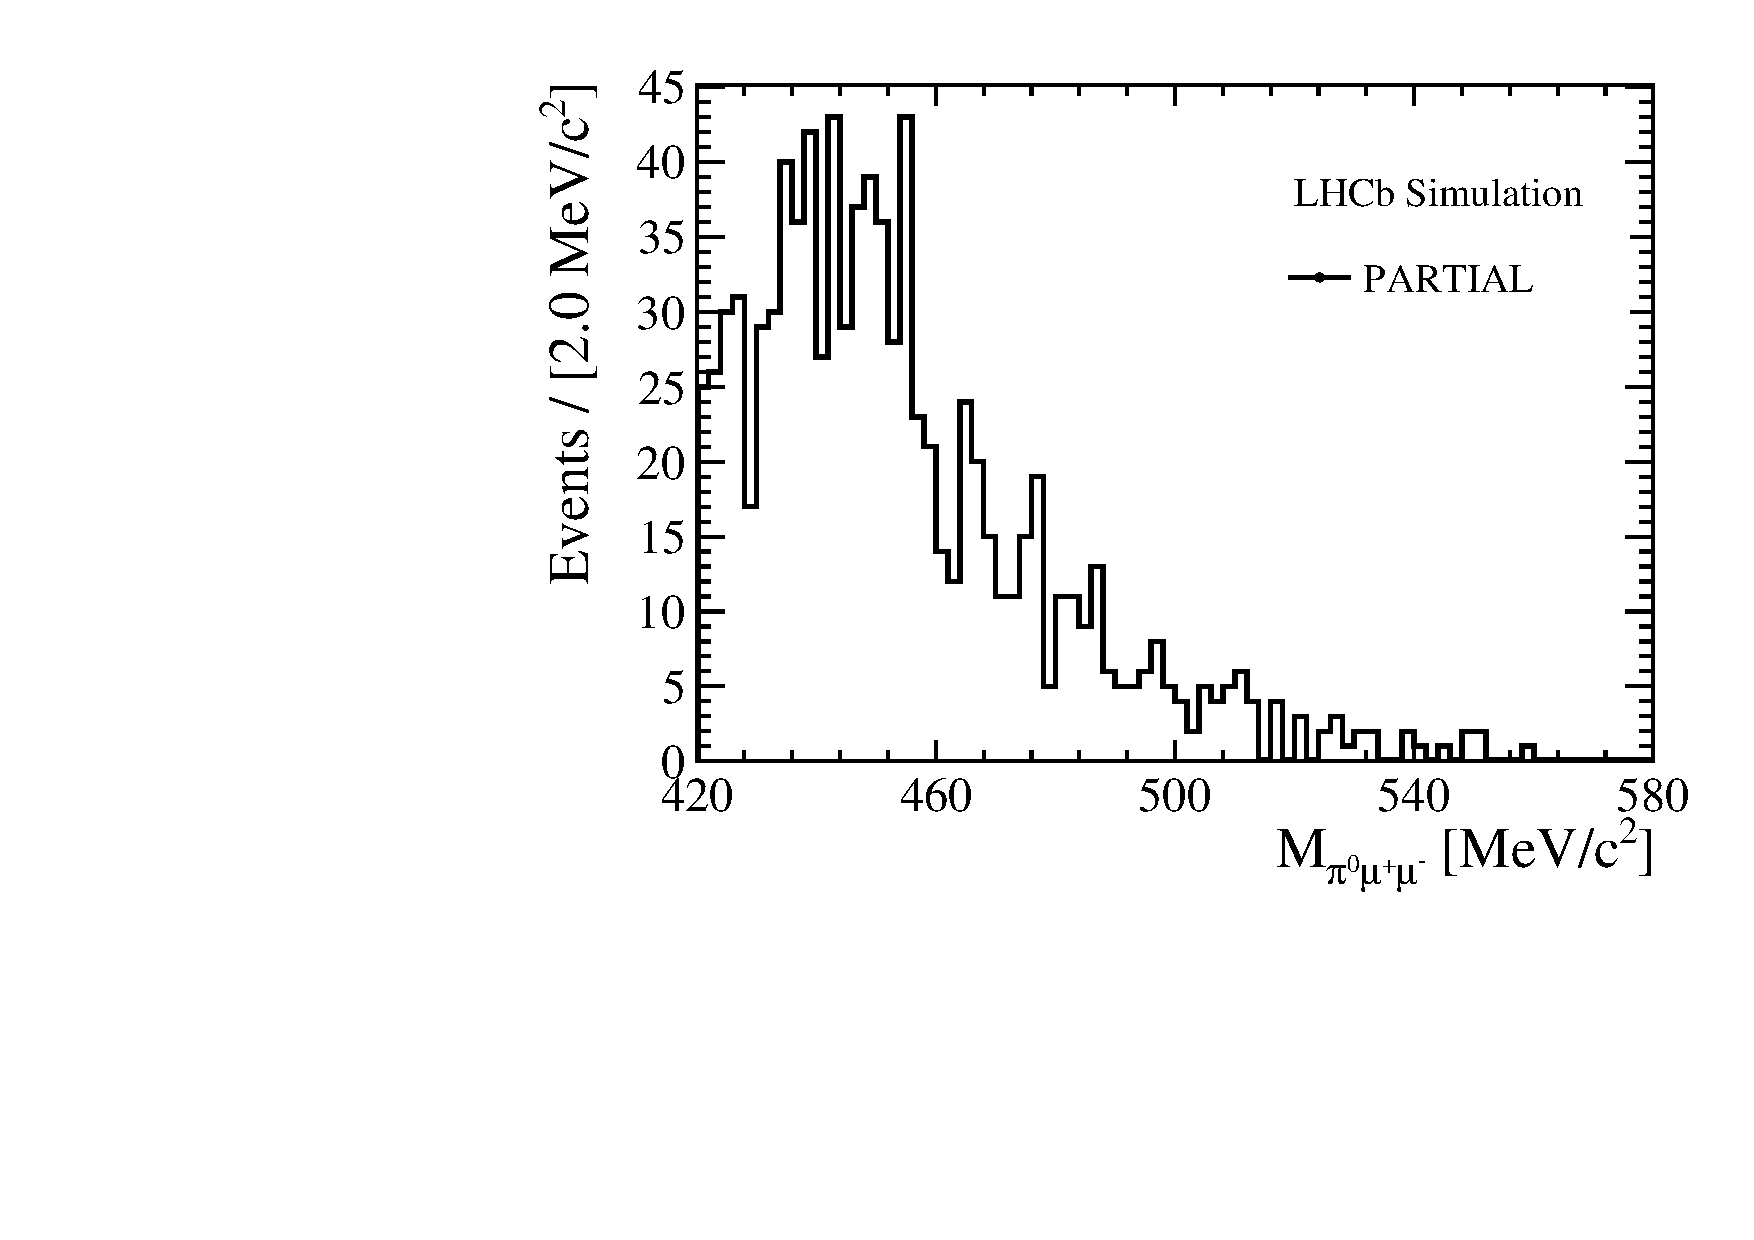
\includegraphics[scale=0.30]{figs/Kspi0MuMu/M_V0_K3pi.pdf}%{figs/mK3pi_PARTIALL.pdf}
\caption{Invariant mass distribution of simulated $K^0\rightarrow\pi^+\pi^-\pi^0$ decays selected in the FULL (left) and PARTIAL (right) categories.  \label{fig:KLTpi}}
\end{center}
\end{figure}

